\documentclass[aspectratio=169,10pt]{beamer}
\usepackage[T1]{fontenc}
\usepackage{lmodern}
\usepackage{amsmath,amssymb}
\usepackage{booktabs}
\usepackage{tikz}
\usetikzlibrary{arrows.meta,positioning,calc}
\usepackage{graphicx}

\definecolor{ink}{HTML}{1D1D20}
\definecolor{acc}{HTML}{B03A2E}
\definecolor{steel}{HTML}{33566E}
\definecolor{pale}{HTML}{F2F0EA}
\definecolor{grey}{HTML}{C9C4BB}

\usetheme{default}
\setbeamertemplate{navigation symbols}{}
\setbeamertemplate{footline}{%
  \hfill{\color{ink!45}\scriptsize\insertframenumber}\hspace*{6mm}\vspace*{3mm}}
\setbeamercolor{frametitle}{fg=ink}
\setbeamercolor{normal text}{fg=ink}
\setbeamercolor{itemize item}{fg=acc}
\setbeamercolor{itemize subitem}{fg=steel}
\setbeamertemplate{itemize item}{\raisebox{0.15em}{\tiny$\blacksquare$}}
\setbeamerfont{frametitle}{size=\Large,series=\bfseries}
\setbeamersize{text margin left=8mm,text margin right=8mm}

\newcommand{\C}{\mathbb{C}}
\newcommand{\ip}[2]{\langle #1|#2\rangle}
\newcommand{\cover}[2]{\begin{columns}[T]\begin{column}{#1}#2\end{column}\end{columns}}

\title{\bfseries Three mutually unbiased bases in $\C^6$}
\subtitle{What a computer-assisted proof claims, what we have checked, and where it stops}
\author{Mathathon working group}
\date{November 2026}

\begin{document}

\begin{frame}[plain]
  \vspace*{6mm}
  {\color{acc}\rule{28mm}{2.2pt}}\\[5mm]
  {\usebeamercolor[fg]{title}\huge\bfseries Three mutually unbiased bases\\[1mm] in $\C^6$\par}
  \vspace{4mm}
  {\large What a computer-assisted proof claims,\\ what we have checked, and where it stops\par}
  \vfill
  {\small Mathathon working group \hfill November 2026\par}
\end{frame}

\begin{frame}{The problem in one picture}
  \begin{columns}[T]
  \begin{column}{0.52\textwidth}
    Two orthonormal bases $B,C$ of $\C^6$ are \emph{mutually unbiased} if
    \[
      \bigl|\ip{b}{c}\bigr|^2=\frac16
      \quad\text{for all } b\in B,\; c\in C .
    \]
    Write $N(d)$ for the largest number of pairwise unbiased bases of $\C^d$.
    \medskip

    \begin{itemize}
      \item Prime powers: $N(d)=d+1$, a complete set.
      \item $d=6$: $N(6)\ge 3$ by $B_1\otimes$ nothing --- from $\C^2\otimes\C^3$.
      \item The upper bound $N(6)\le 3$ is the dimension-six MUB conjecture --- attributed to
            Zauner, open for twenty years.
    \end{itemize}
  \end{column}
  \begin{column}{0.46\textwidth}
    \centering
    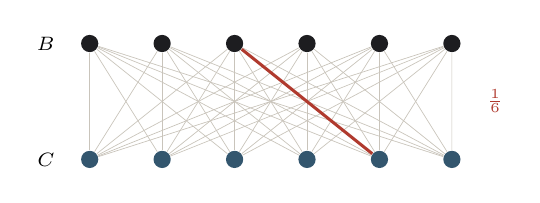
\begin{tikzpicture}[scale=0.92]
      % two bases: 6 dots each, all cross overlaps 1/sqrt6
      \foreach \i in {0,...,5}{
        \node[circle,fill=ink,inner sep=2.2pt] (a\i) at (\i,1.6) {};
        \node[circle,fill=steel,inner sep=2.2pt] (b\i) at (\i,0) {};
      }
      \foreach \i in {0,...,5}{\foreach \j in {0,...,5}{
        \draw[grey,line width=0.25pt] (a\i)--(b\j);}}
      \draw[acc,line width=1.1pt] (a2)--(b4);
      \node[acc,font=\scriptsize,right] at (5.35,0.8) {$\tfrac16$};
      \node[font=\scriptsize,left] at (-0.35,1.6) {$B$};
      \node[font=\scriptsize,left] at (-0.35,0) {$C$};
    \end{tikzpicture}

    \vspace{4mm}
    {\small\color{ink!70} every entry of the $6\times6$ table of overlaps has modulus $1/\sqrt6$}
  \end{column}
  \end{columns}
\end{frame}

\begin{frame}{Why dimension six}
  \begin{itemize}
    \item $d=2,3,4,5$: complete sets exist ($d+1$ bases), because $d$ is a prime power.
    \item $d=6$: no prime power, so the construction says nothing. It has been the smallest
          open case for two decades; $3\le N(6)\le 7$ was all that was known.
    \item The obstruction is \emph{not} arithmetic. It is the geometry of a $45$-dimensional
          torus of phases, and it is now claimed to be settled by a finite computation.
  \end{itemize}
  \vspace{3mm}
  \begin{block}{}
    \centering
    \textbf{Theorem (OpenAI preprint, 24 Sep 2026, computer-assisted).}
    There are no four pairwise mutually unbiased bases in $\C^6$. With the tensor
    construction, $N(6)=3$.
  \end{block}
  \vspace{1mm}
  {\small\color{ink!70}The whole talk is about what ``computer-assisted'' costs, and what it buys.}
\end{frame}

\begin{frame}{Step 0: one unitary, and the problem becomes a matrix of phases}
  Normalise $B_1$ to the coordinate basis. Then $B_2$ is the column set of $H/\sqrt6$ with
  \[
    |H_{jk}|=1,\qquad HH^{*}=6I ,
  \]
  a \emph{complex Hadamard matrix}. Row and column rephasings are gauge, so $11$ of the $36$
  phases can be set to $1$: \textbf{25 phases matter}.
  \medskip

  \begin{columns}[T]
    \begin{column}{0.46\textwidth}
      \centering
      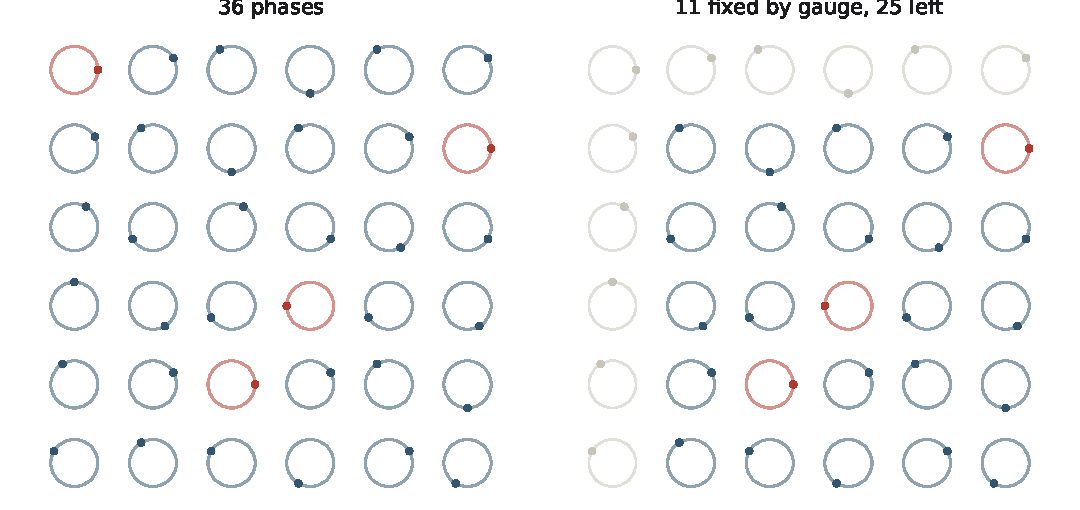
\includegraphics[width=0.92\textwidth]{figs/fig_phases.pdf}
    \end{column}
    \begin{column}{0.52\textwidth}
      \small
      Two rephasing moves are free:
      \[
        H\mapsto D_r H D_c ,\qquad |D_r|=|D_c|=1 .
      \]
      Dephasing sets row $0$ and column $0$ to $1$; a further $Z_6$ acts on the remaining block.
      \medskip

      The job: exclude two further bases for \emph{every} such $H$ --- not for one family.
      That quantifier is the new content.
    \end{column}
  \end{columns}
\end{frame}

\begin{frame}{The proof is one cover, in five stages}
  \centering
  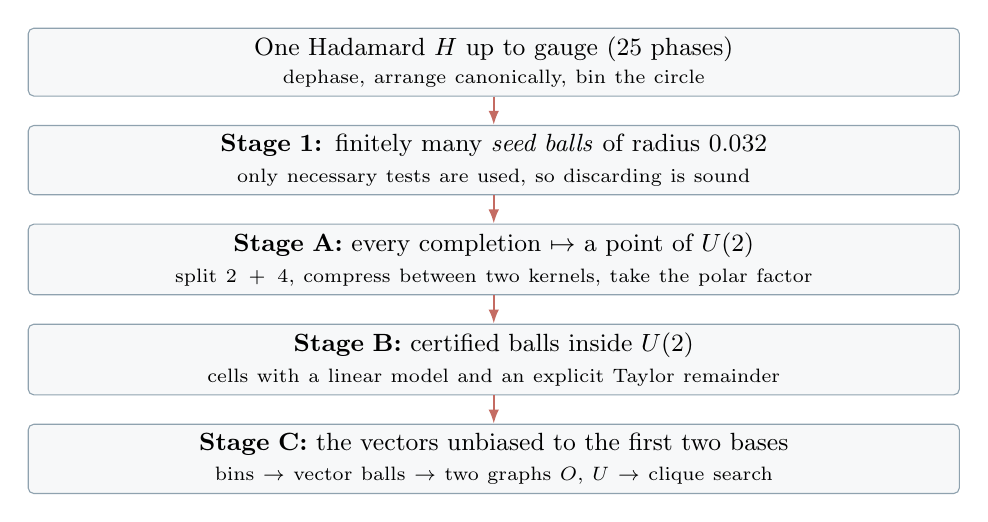
\begin{tikzpicture}[node distance=3.6mm,font=\small,
    box/.style={draw=steel!55,fill=steel!4,rounded corners=2pt,text width=11.6cm,
                align=center,inner sep=3.2pt,minimum height=8.2mm},
    ar/.style={-{Latex[length=1.8mm]},thick,acc!75}]
    \node[box] (a) {One Hadamard $H$ up to gauge (25 phases)\\[-1pt]
      \scriptsize dephase, arrange canonically, bin the circle};
    \node[box,below=of a] (b) {\textbf{Stage 1:} finitely many \emph{seed balls} of radius $0.032$\\
      \scriptsize only necessary tests are used, so discarding is sound};
    \node[box,below=of b] (c) {\textbf{Stage A:} every completion $\mapsto$ a point of $U(2)$\\
      \scriptsize split $2+4$, compress between two kernels, take the polar factor};
    \node[box,below=of c] (d) {\textbf{Stage B:} certified balls inside $U(2)$\\
      \scriptsize cells with a linear model and an explicit Taylor remainder};
    \node[box,below=of d] (e) {\textbf{Stage C:} the vectors unbiased to the first two bases\\
      \scriptsize bins $\to$ vector balls $\to$ two graphs $O$, $U$ $\to$ clique search};
    \foreach \x/\y in {a/b,b/c,c/d,d/e} \draw[ar] (\x) -- (\y);
  \end{tikzpicture}

  \vspace{2mm}
  {\small\color{ink!70}Each arrow is a \emph{cover}: the next stage keeps every exact candidate the previous one could produce.}
\end{frame}

\begin{frame}{Stage 1: a finite cover of all second bases}
  \begin{columns}[T]
  \begin{column}{0.56\textwidth}
    \small
    Lemma 2.4 puts every $H$ into a canonical form with a \emph{nine-phase seed}. Each of the nine
    phases is binned at $N=112$: width $w=1/112$, radius $R=0.032$ cycles.
    \medskip

    \begin{tabular}{@{}lr@{}}
      \toprule
      bin pairs tested & $151{,}744{,}086$\\
      centres retained & $249{,}878$\\
      \bottomrule
    \end{tabular}
    \medskip

    A pair of bins is dropped only when a \emph{necessary} inequality fails on the whole box:
    gap bounds, a Taylor test on the two vanishing sums, and a shared-coordinate
    intersection. No sampling.
  \end{column}
  \begin{column}{0.42\textwidth}
    \centering
    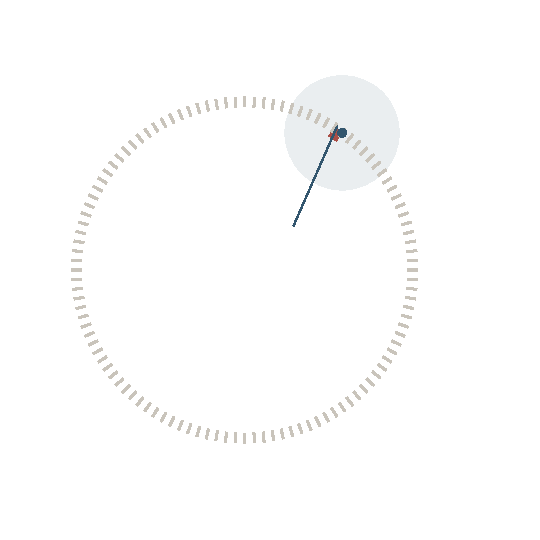
\includegraphics[width=0.86\textwidth]{figs/fig_cover.pdf}\\[1mm]
    {\scriptsize\color{ink!65} one bin, and the ball that covers it (radius exaggerated)}
  \end{column}
  \end{columns}
\end{frame}

\begin{frame}{Stage A: a $6\times6$ unknown collapses to $U(2)$}
  \begin{columns}[T]
  \begin{column}{0.5\textwidth}
    \small
    Split $H$ into $2+4$ blocks at a seed centre. The two off-diagonal blocks have rank $2$
    at the centre, so their kernels are fixed \emph{for the whole seed ball}.
    \medskip

    Compress the unknown $4\times4$ block between them:
    \[
      Y=K_C^{*}D'K_B,\qquad 6I-Y^{*}Y\succeq0,\quad \operatorname{tr}(6I-Y^*Y)\le q<0.32 .
    \]
    Then the polar factor $V\in U(2)$ exists and
    \[
      \|Y-\sqrt6\,V\|_F\le p .
    \]
    \medskip
    Every completion of the seed is a point of $U(2)$ --- a four-angle chart with cells.
  \end{column}
  \begin{column}{0.46\textwidth}
    \centering
    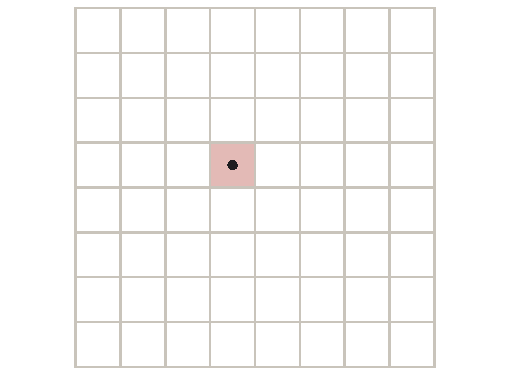
\includegraphics[width=0.72\textwidth]{figs/fig_chart.pdf}\\[1mm]
    {\scriptsize\color{ink!65} $U(2)$ cut into cells; the completion lands in one of them}\\[3mm]
    {\small $N_u=16\to32\to64\to\dots\to512$}
  \end{column}
  \end{columns}
\end{frame}

\begin{frame}{Stage B: shrink each ball until it is small}
  \small
  A \emph{Root certificate} is a centre $P$, a numerical tangent frame $T$, and constants such that
  every exact completion $\delta$ satisfies
  \[
    \|(I-TT^{*})\delta\|\le n_0+id\,s+Cs^2,\qquad s=\|\delta\| .
  \]
  Refining in tangent coordinates turns radius $\approx0.125$ into three passes:
  \[
    (\tau,w)=(0.07,\,0.013)\;\longrightarrow\;(0.016,\,0.005)\;\longrightarrow\;(0.011,\,0.0038).
  \]
  \medskip
  \begin{itemize}
    \item Nothing here needs a contraction or a fixed point: the bound is a monotone iteration.
    \item A parent that fails to refine stays on the books as an \emph{obligation}, never as a pass.
  \end{itemize}
  \vspace{2mm}
  {\color{ink!70}This is where most of the machine time goes, and where the picture of ``a ball around a matrix'' becomes usable.}
\end{frame}

\begin{frame}{Stage C: inside a ball, count cliques}
  \begin{columns}[T]
  \begin{column}{0.5\textwidth}
    \small
    Vectors unbiased to the first base are $e(\beta)/\sqrt6$: five phases. Bin them
    ($12\to24\to48\to96$), cluster into closed vector balls, and build two graphs:
    \medskip

    \begin{itemize}
      \item $O$: orthogonality not excluded.
      \item $U$: unbiasedness not excluded.
    \end{itemize}
    \medskip
    Two further bases force two disjoint $6$-cliques of $O$ whose $36$ cross pairs are all in $U$.
    The search decides whether that pattern exists. If it does not, the ball is excluded ---
    a genuine exclusion, because $O,U$ are supersets of the truth.
  \end{column}
  \begin{column}{0.46\textwidth}
    \centering
    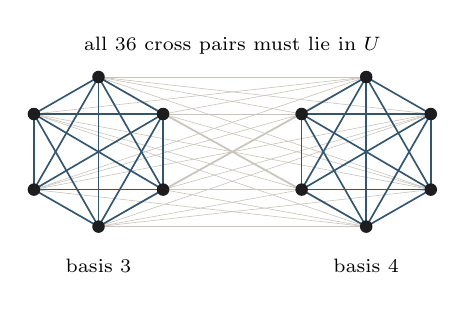
\begin{tikzpicture}[font=\scriptsize,dot/.style={circle,fill=ink,inner sep=1.6pt}]
      \foreach \k/\dx in {L/0,R/3.4}{
        \coordinate (\k1) at (\dx+0,0.95); \coordinate (\k2) at (\dx-0.82,0.48);
        \coordinate (\k3) at (\dx-0.82,-0.48); \coordinate (\k4) at (\dx+0,-0.95);
        \coordinate (\k5) at (\dx+0.82,-0.48); \coordinate (\k6) at (\dx+0.82,0.48);}
      \foreach \i in {1,...,6}{\foreach \j in {1,...,6}{\draw[grey,line width=0.22pt] (L\i)--(R\j);}}
      \foreach \k in {L,R}{\foreach \i/\j in {1/2,1/3,1/4,1/5,1/6,2/3,2/4,2/5,2/6,3/4,3/5,3/6,4/5,4/6,5/6}{
        \draw[steel,line width=0.6pt] (\k\i)--(\k\j);}}
      \foreach \k in {L,R}{\foreach \i in {1,...,6}{\node[dot] at (\k\i) {};}}
      \node at (1.7,1.35) {all $36$ cross pairs must lie in $U$};
      \node at (0,-1.45) {basis 3}; \node at (3.4,-1.45) {basis 4};
    \end{tikzpicture}
  \end{column}
  \end{columns}
\end{frame}

\begin{frame}{The same test, on one worked pair}
  \begin{columns}[T]
  \begin{column}{0.56\textwidth}
    \small
    Standard $+$ Fourier pair in $\C^6$. Enumerate every ray on the $12$th-root lattice that is
    unbiased to both: $12$ rays (exact, $\mathbb{Z}[\zeta_{12}]$).
    \medskip

    Then decide the two integer tests for all $\binom{12}{2}=66$ pairs:
    \[
      \textstyle\sum_k z^{a_k-b_k}=0 \;\; (O),\qquad
      \bigl|\textstyle\sum_k z^{a_k-b_k}\bigr|^2=6 \;\; (U).
    \]
    \medskip
    Four candidate bases emerge; none is unbiased to any other; the pattern needed for two further
    bases is absent.
  \end{column}
  \begin{column}{0.42\textwidth}
    \centering
    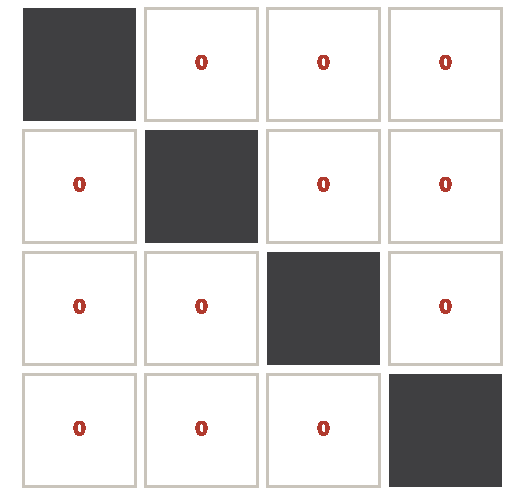
\includegraphics[width=0.78\textwidth]{figs/fig_sextuples.pdf}\\[1mm]
    {\scriptsize\color{ink!65} four candidate bases (dark diagonal); every off-diagonal entry counts
    unbiased cross pairs, and all are zero}
  \end{column}
  \end{columns}
\end{frame}

\begin{frame}[plain]
  \begin{columns}[c]
  \begin{column}{0.55\textwidth}
    \vspace*{4mm}
    {\color{acc}\rule{22mm}{2pt}}\\[3mm]
    {\Large\bfseries Discarding the candidates}\\[2mm]
    {\small forty-five seconds of the actual program, unedited: the exact integer tests,
    the tally, and a sanity check that the verdict has margin.}
    \bigskip

    \begin{tabular}{@{}ll@{}}
      \small\color{ink!70}\textbf{file} & \small\texttt{slides/video/stageC-demo.mp4}\\
      \small\color{ink!70}\textbf{code} & \small\texttt{examples/step4\_example.py}\\
      \small\color{ink!70}\textbf{runtime} & \small 0.13\,s\\
    \end{tabular}
  \end{column}
  \begin{column}{0.43\textwidth}
    \centering
    \begin{tikzpicture}
      \node[inner sep=0] (p) {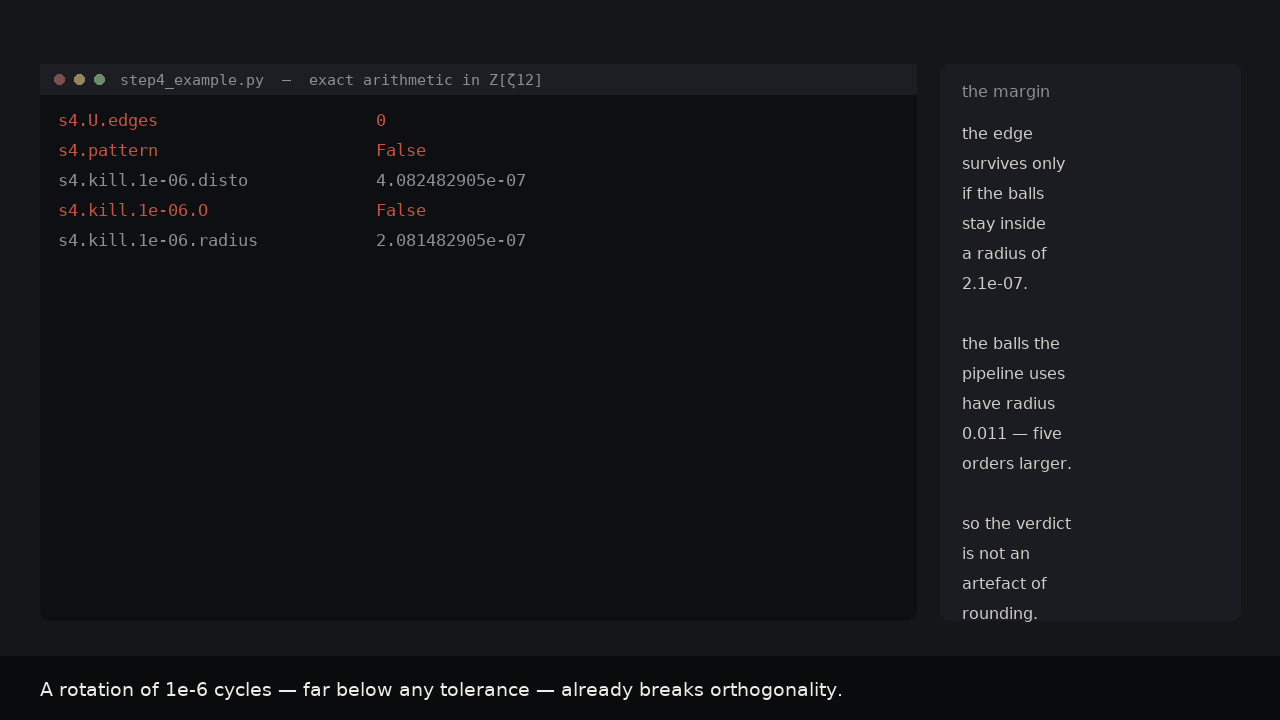
\includegraphics[width=\textwidth]{video/poster.png}};
      \draw[white,line width=1.2pt,fill=white,fill opacity=0.85] (p.center) ++(-6mm,0) -- ++(12mm,7mm) -- ++(0,-14mm) -- cycle;
    \end{tikzpicture}
  \end{column}
  \end{columns}
\end{frame}

\begin{frame}{Stage 5: the ledger, and where the claim lives}
  \small
  Every record of the run has one of three states: \emph{excluded}, \emph{refined into
  children}, or \emph{unresolved}. The theorem is the statement that the third column is empty.
  \medskip

  \begin{columns}[T]
  \begin{column}{0.52\textwidth}
    \begin{tabular}{@{}lr@{}}
      \toprule
      Stage-C records & $23{,}506$\\
      \quad excluded: no pattern & $23{,}343$\\
      \quad hit the $5\cdot10^6$ step cap & $163$\\
      \midrule
      graph steps & $3{,}747{,}019{,}119$\\
      $O+U$ edges built & $368{,}119{,}692$\\
      \bottomrule
    \end{tabular}
  \end{column}
  \begin{column}{0.44\textwidth}
    
\includegraphics[width=\textwidth]{figs/fig_ledger.pdf}\\[2mm]
    {\scriptsize\color{ink!65} the $163$ capped records are resolved by a second policy in the
    fallback pass, not inside Stage C. A capped search is \emph{unresolved}; it is never a negative.}
  \end{column}
  \end{columns}
  \vspace{2mm}
  \begin{block}{}
    \small\textbf{Theorem 7.1} turns ``all terminal conditions of the specified invocation script
    hold, with record provenance and batch checks'' into ``no four MUBs in $\C^6$''.
  \end{block}
\end{frame}

\begin{frame}{What the claim rests on}
  \small
  The mathematical content is the collection of \emph{necessity} lemmas. Sufficiency --- that the
  search actually closes --- is not proved; it is observed. Three things must hold.
  \medskip

  \begin{enumerate}
    \item \textbf{Arithmetic.} Every certificate evaluation is binary64, with $\sim$20 pages of
          one-sided absolute-error budgets (Appendix A) and a build that is \texttt{-march=native}.
          A different compiler is a different experiment.
    \item \textbf{Execution.} Seven unchanged C++ sources, $100$ invocations, about $75$ minutes,
          archived records with SHA-256s. The hypothesis is an \emph{event}, not an inequality a
          reader can check.
    \item \textbf{Fidelity.} That the sources implement the specification the lemmas describe.
          The paper states the contracts in prose; no code appears in it.
  \end{enumerate}
  \vspace{2mm}
  {\color{acc}\textbf{And one design principle worth keeping:}} a proposal (a centre, a frame, a
  direction) is used only after an independent one-sided check with explicit slack. Anything not
  certified becomes \emph{unresolved}, and \textbf{unresolved is never negative}.
\end{frame}

\begin{frame}{What we have checked ourselves}
  \small
  \begin{columns}[T]
  \begin{column}{0.55\textwidth}
    \begin{itemize}\footnotesize\setlength{\itemsep}{0.8mm}
      \item \textbf{The covering step, reproduced.} An independent implementation emits
            \texttt{centers.txt} byte for byte: $7{,}339{,}546$\,B, $249{,}878$ centres,
            same SHA-256, $400.8$\,s against the published $401.8$\,s.
      \item \textbf{Seed certificate:} $151{,}744{,}086$ pair records, $151{,}742{,}926$ mandatory
            covers, zero missing pairs, zero undecided dual comparisons.
      \item \textbf{Stage C:} $269{,}403$ basic-predicate evaluations and $61{,}832$ joint
            comparisons re-checked exactly or outwards on four complete batch records;
            $10{,}293$ exclusions, no retained pair violated.
      \item \textbf{Stage B:} a complete transported-frame cover of one parent, two arithmetic routes.
      \item \textbf{Stage A:} exact subdivision trees and twenty directional certificates on real
            cells. \textbf{Root witnesses:} $34$ formerly anomalous records plus the two
            stored-tensor failures.
      \item \textbf{Assembly:} the six stage interfaces composed in Lean --- conditionally.
    \end{itemize}
  \end{column}
  \begin{column}{0.42\textwidth}
    \begin{block}{}
      \small We do \emph{not} claim the global execution is certified, and we do not claim
      $N(6)=3$ has been proved by this work.
    \end{block}
    \vspace{2mm}
    {\scriptsize\color{ink!70} The verified fragments are useful on their own: they turn opaque
    binary64 decisions into small arithmetic facts, and they isolate what is left.}
  \end{column}
  \end{columns}
\end{frame}

\begin{frame}{What the audit changed}
  \small
  None of these is a hole in the argument. All of them are holes in the evidence
  \emph{interface} --- which is exactly what a reader cannot see.
  \medskip

  \begin{itemize}\setlength{\itemsep}{2.2mm}
    \item \textbf{The $112$ bins are not justified as stated.} Coverage needs $N\ge47$,
          \texttt{int8\_t} forces $N\le128$, and $112$ sits arbitrarily between them. The real
          constraint set is coverage, integer width and bucket reuse.
    \item \textbf{The stated tangent dimension $k\le10$ is unreachable} under the
          $5\cdot10^7$-box cap: in practice $k\le5,5,7$. A $k=6$ record would fail its parent while
          the run reports no bad parent.
    \item \textbf{The composition index was wrong.} \texttt{fine\_index} held
          \texttt{256*batch+batch\_index}, so only $14$ of the $163$ capped parents matched a capped
          record; rebuilt from the manifest, $1{,}127$ children and $11{,}838$ incidences preserved.
    \item \textbf{\texttt{g0.txt} looked like a broken relabelling.} It decodes big-endian and is a
          valid one --- under eight ball permutations, not a unique one.
    \item \textbf{Stage-C cutoff.} The radius $(\cdot042-1.11w)^2$ has a negative base for $M<26$;
          inert in the run, but wrong as a formula.
  \end{itemize}
\end{frame}

\begin{frame}{Extension: you cannot even add one vector}
  \begin{columns}[T]
  \begin{column}{0.52\textwidth}
    \small
    Let $B_1,B_2,B_3$ be a MUB triple in $\C^6$, and call $v$ \emph{admissible} if it is unbiased to
    all three. A fourth basis needs six mutually orthogonal admissible vectors.
    \medskip

    \textbf{Count.} Dephase so the triple is critical: $s=2(d-1)=10$ vectors in the last two groups
    carry $p=(d-1)(s-1)=45$ phases, and unbiasedness imposes $c=\binom{s}{2}=45$ conditions ---
    a $45$-torus cut to isolated points.
    \medskip

    One more vector adds $5$ phases but $10$ conditions. The system is overdetermined by five,
    and every further vector costs five more.
    \medskip

    {\color{acc}\textbf{Claim:} for every triple decided so far, no admissible vector exists;
    $k_{\max}=0$. The classification of all triples in $\C^6$ is cited from Wuttig--Tindall
    (arXiv:2611.06917), not re-verified here.}
  \end{column}
  \begin{column}{0.44\textwidth}
    \small
    \textbf{Mechanism.} Fix the standard and Fourier bases. Exactly $48$ rays are unbiased to both
    (Grassl 2004); each is unbiased to $4$ or $12$ others, giving $300$ unbiased pairs and exactly
    $16$ orthonormal sextuples. None of the $16$ is unbiased to any other.
    \medskip

    \textbf{Not a corollary of $N(6)=3$.} In $\C^4$ five MUBs exist, yet the $Z_4$-Weyl triple has
    $k=0$ while a triple inside the five has $k=4$. ``No fourth basis'' does not forbid a single
    extra vector --- here, nothing does.
  \end{column}
  \end{columns}
\end{frame}

\begin{frame}{Extensions: the edges of the result}
  \small
  \begin{description}
    \item[Four bases in $\C^6$.] Excluded by the theorem. The exclusion is quantifier-level: it
      covers \emph{all} complex Hadamard second bases, not one family. Earlier work covered the
      Fourier family only.
    \item[How far from four?] Approximate MUBs: $0<\varepsilon_6^{*}\le0.030224240773$, certified in
      exact rational arithmetic. Inside the product class $\C^2\otimes\C^3$ the optimum is exactly
      $1/18$. No two-body inequality can give a positive lower bound --- a structural limit, not a
      gap in technique.
    \item[Strata.] The order-three stratum carries a numerical no-quartet deficit
      $\Delta\ge0.0422687212$; one open statement (symmetry propagation) remains.
    \item[Better certificates.] The cell body's support function gives an optimal direction
      $y^{*}=c-\mathrm{Proj}_K(c)$ and a merged certificate $13.8\%$ better in the median --- inert
      at the boundary, as expected.
    \item[An elegant proof?] Not found. The monodromy route is dead: off a discriminant the count is
      locally constant, so no proper closed discriminant can separate.
  \end{description}
\end{frame}

\begin{frame}{What it means for quantum information}
  \small
  {\footnotesize\color{ink!60}Four statements that survive a check against primary sources. The
  preprint itself makes no quantum-information claim; the framing is ours.}
  \vspace{1mm}
  \begin{itemize}\setlength{\itemsep}{2.2mm}
    \item \textbf{Tomography.} A state in $\C^6$ has $35$ real parameters; one orthonormal basis
      fixes $5$, so $7$ settings is the minimum. A complete MUB set minimises the statistical error
      among seven-setting schemes (Wootters--Fields 1989; scope: Durt et al. 2010, \S4.2).
      Three MUBs fix $15$ of the $35$ --- the optimal MUB scheme is unavailable.
    \item \textbf{Uncertainty.} The strong state-independent bound averages over a \emph{complete}
      MUB set (Ivanovi\'c 1992; S\'anchez 1993; S\'anchez-Ruiz 1995), needing $d+1=7$ bases here.
      With three, only the pairwise consequence survives: $\frac1L\sum_j H(B_j)\ge\frac12\log_2 6
      =1.292$ bits. Mutual unbiasedness alone does not give strength (Ballester--Wehner 2007).
    \item \textbf{Key distribution is unharmed.} The six-dimensional analogue of the six-state
      protocol would be a seven-MUB protocol, hence cannot exist. The two-basis qudit protocol is
      untouched: Cerf et al.\ (2002) allow $\approx22.5\%$ error at $d=6$ from one complementary
      pair.
    \item \textbf{A closure, not a capability.} Nothing is enabled; capacities that do not count
      MUBs are unchanged --- dense coding still gives $2\log_2 6=5.17$ bits per six-level system
      (Durt et al.\ \S3.2; Hiroshima 2001).
  \end{itemize}
\end{frame}

\begin{frame}{Where this leaves the problem}
  \small
  \begin{columns}[T]
  \begin{column}{0.48\textwidth}
    \textbf{Settled}
    \begin{itemize}
      \item No four MUBs in $\C^6$, conditional on one documented binary64 run.
      \item No admissible vector on any decided triple: $k_{\max}=0$.
      \item The covering step, reproduced from scratch, byte-identical.
      \item A verified core: seed cover, four Stage-C batches, one Stage-B parent, Stage-A cells,
            Root witnesses.
    \end{itemize}
  \end{column}
  \begin{column}{0.48\textwidth}
    \textbf{Open}
    \begin{itemize}
      \item A small checker that consumes the record stream and re-verifies each inequality,
            so the conclusion rests on a certificate rather than on an event.
      \item Outward-rounded arithmetic, which would delete Appendix A and the compiler dependence.
      \item $d=4$ controls: the same pipeline must \emph{fail} to exclude a fourth basis.
      \item Stage A/B/C certification beyond the fragments; the Lean assembly is conditional and
            stops at $N(6)\le5$.
    \end{itemize}
  \end{column}
  \end{columns}
  \vfill
  \begin{center}
    {\color{acc}\rule{30mm}{1.6pt}}\\[2mm]
    {\small The interesting claim is not the number. It is that a finite, checkable object can
    carry an exclusion over a $45$-torus of phases --- and that we can say exactly how much of it
    has been checked.}
  \end{center}
\end{frame}

\end{document}
